\selectlanguage{italian}

La trattazione degli atomi a molti elettroni (Many-Electron Atoms) è resa non banale dall'interazione elettrone-elettrone, la quale rende impossibile la risoluzione esatta del problema\footnotemark. È dunque necessario adottare alcune semplificazioni.

\footnotetext{La funzione d'onda di ciascun elettrone dipende da tre variabili spaziali, dunque, discretizzando ciascuna di esse in una griglia di 10 numeri reali, la descrizione di un sistema a $ N $ elettroni richiede di trattare $ (10^3)^N $ numeri reali: già per $ N = 4 $ ciò necessiterebbe di qualche Tb, mentre per $ N = 27 $ si raggiunge l'ordine di grandezza del numero totale di atomi nell'Universo. La trattazione numerica del problema è dunque impossibile.}

\section{Approssimazione a particelle indipendenti}

È possibile trovare soluzioni approssimate per MEAs costruendo il relativo spazio di Hilbert a partire dagli stati single-particle.

\subsection{Particelle identiche}

Gli elettroni sono particelle indistinguibili tra loro, dunque è necessario ricordare le proprietà dei sistemi quantistici di particelle identiche. \\
Dato un sistema di $ N $ particelle identiche, ciascuna descritta da uno spazio di Hilbert $ \hilb $, il sistema totale sarà descritto da un sottospazio del prodotto diretto di tali spazi. In particolare, definendo l'operatore di scambio $ \pi_{ij} $ che scambia le particelle $ i \leftrightarrow j $, dato che $ \pi_{ij}^2 = \id $ si ha che i suoi autovalori possibili sono $ \pm 1 $: stati $ \pi_{ij} \ket{\psi} = + \ket{\psi} $ sono detti \textit{stati bosonici}, sono simmetrici per scambio di particelle e descrivono sistemi di spin intero; stati $ \pi_{ij} \ket{\psi} = - \ket{\psi} $ sono detti \textit{stati fermionici}, sono antisimmetrici per scambio di particelle e descrivono sistemi di spin semi-intero. La definizione degli stati bosonici/fermionici a partire dagli stati single-particle è dunque data rispettivamente da:
\begin{equation}
	\ket{\alpha_1 , \dots , \alpha_N}^\text{(s)} \defeq \frac{1}{\sqrt{N!}} \sum_{\pi \in S^N} \ket{\alpha_{\pi(1)} , \dots , \alpha_{\pi(N)}}
\end{equation}
\begin{equation}
	\ket{\alpha_1 , \dots , \alpha_N}^\text{(a)} \defeq \frac{1}{\sqrt{N!}} \sum_{\pi \in S^N} (-1)^{\{\pi\}} \ket{\alpha_{\pi(1)} , \dots , \alpha_{\pi(N)}}
\end{equation}
dove $ \{\pi\} $ è il carattere della permutazione e $ \alpha_n $ indica il set completo di quantum numbers dell'$ n $-esima particella. Come si può vedere, il principio d'esclusione di Pauli discende banalmente da queste definizioni: un sistema bosonico non ha restrizioni sui quantum numbers dei singoli bosoni che lo compongono, mentre un sistema fermionico, dato il fattore $ (-1)^{\{\pi\}} $, risulta avere $ \ket{\psi} = 0 $ se si considerano due fermioni con gli stessi quantum numbers.

\begin{example}{Identicità degli atomi}{}
	Si consideri un atomo di $ \ch{^3He} $: esso è composto da 2 protoni, 1 neutrone e 2 elettroni, dunque overall è un sistema fermionico: se si scambiano tra loro due tali atomi, si ottiene un fattore $ (-1)\cdot(-1) = +1 $ per i protoni, idem per gli elettroni, e $ (-1) $ per i neutroni, risultando in un fattore totale $ (-1) $. \\
	D'altro canto, un atomo di $ \ch{^{238}U} $, composto da 92 protoni, 146 neutroni e 92 elettroni, è un sistema bosonico per un ragionamento analogo. \\
	In generale, atomi con $ A + Z $ pari sono bosoni, mentre atomi con $ A + Z $ dispari sono fermioni.
\end{example}

L'antisimmetria per scambio dei sistemi a molti elettroni ne condiziona fortemente la dinamica, in quanto la repulsione tra elettroni data dall'antisimettrizzazione della funzione d'onda è spesso più efficace della repulsione elettromagnetica tra di essi: senza antisimmetria, gli elettroni nel ground state occuperebbero tutti la shell $ \text{1s} $.

\subsubsection{Funzione d'onda fermionica}

Si consideri un sistema di $ N $ fermioni, ciascuno descritto da uno spazio di Hilbert con ket base $ \ket{w_n} = \ket{\ve{r}_n , \sigma_n} $ di posizione e spin.

\begin{theorem}{Determinante di Slater}{}
	La base dello spazio di Hilbert di un sistema di $ N $ fermioni è data dal \textit{determinante di Slater}:
	\begin{equation}
		\Psi_{\alpha_1 , \dots , \alpha_N}(w_1 , \dots , w_N) = \frac{1}{\sqrt{N!}}
		\begin{vmatrix}
			\psi_{\alpha_1}(w_1) & \dots & \psi_{\alpha_1}(w_N) \\
			\vdots & \ddots & \vdots \\
			\psi_{\alpha_N}(w_1) & \dots & \psi_{\alpha_N}(w_N)
		\end{vmatrix}
	\end{equation}

	\tcblower

	\begin{proof}
		Essendo lo spazio di Hilbert totale $ \hilb^\text{(a)} $, la funzione d'onda dello stato fermionico generico $ \ket{\alpha_1 , \dots , \alpha_N}^\text{(a)} $ sarà:
		\begin{equation*}
			\begin{split}
				\Psi_{\alpha_1 , \dots , \alpha_N}(w_1 , \dots , w_N)
				& = {^\text{(a)}\langle}w_1 , \dots , w_N | \alpha_1 , \dots , \alpha_N{\rangle^\text{(a)}} \\
				& = \frac{1}{N!} \sum_{\pi,\rho \in S^N} (-1)^{\{\pi\}} (-1)^{\{\rho\}} \braket{w_{\rho(1)} , \dots , w_{\rho(N)} | \alpha_{\pi(1)} , \dots , \alpha_{\pi(N)}} \\
				& = \sum_{\pi \in S^N} (-1)^{\{\pi\}} \frac{1}{N!} \sum_{\rho \in S^N} (-1)^{\{\rho\}} \psi_{\alpha_{\pi(1)}}(w_{\rho(1)}) \dots \psi_{\alpha_{\pi(N)}}(w_{\rho(N)}) \\
				& = \sum_{\pi \in S^n} (-1)^{\{\pi\}} \psi_{\alpha_{\pi(1)}}(w_1) \dots \psi_{\alpha_{\pi(N)}}(w_N)
			\end{split}
		\end{equation*}
		Questa è proprio la definizione di determinante della matrice $ A_{ij} = \psi_{\alpha_i}(w_j) $. Aggiungendo un fattore di normalizzazione $ (N!)^{-1/2} $ si ottiene la tesi\footnote{Ciò permette di usare come dominio d'integrazione tutto lo spazio di definizione delle $ w_n $, e non solo l'iper-triangolo $ w_1 > \dots > w_n $.}.
	\end{proof}
\end{theorem}

In questo modo diventa possibile trattare numericamente il problema\footnotemark. La complessità del problema viene relegata ai coefficienti dell'espansione dello stato generico su tale base:
\begin{equation}
	\ket{\Psi} = \sum_{\alpha_1 , \dots , \alpha_N} c_{\alpha_1 , \dots , \alpha_N} \ket{\alpha_1 , \dots , \alpha_N}^\text{(a)}
\end{equation}
con $ c_{\alpha_1 , \dots , \alpha_N} \in \C $. In questo modo, dunque, si ottiene lo stato del sistema totale a partire dagli stati single-particle: da qui l'\textit{approssimazione a particelle indipendenti}.

\footnotetext{I ket di base ottenuti tramite il determinante di Slater contengono una quantità d'informazione che, seguendo l'esempio della nota precedente, scala come $ N \cdot 10^3 $, dunque linearmente.}

\subsection{Elettroni non-interagenti}

Si consideri il potenziale d'interazione elettrone-elettrone $ V_{ee} $ completamente trascurabile: in tal caso, il problema ad $ N $ elettroni si fattorizza completamente, poiché ciascun elettrone si muove indipendentemente dagli altri nel potenziale $ V_{ne} $. Trascurando gli effetti relativistici, gli autostati dei singoli elettroni sono rappresentati dalla funzione d'onda idrogenoide\footnotemark: si ha dunque $ \alpha_i \equiv \{n_i, \ell_i, m_i, m_{s_i}\} $.

\footnotetext{Nel caso dei MEAs, si può ignorare la dimensione finita del nucleo, assumendo $ \mu \equiv m_e $ e $ a \equiv a_0 $.}

\begin{example}{Notazione spettroscopica}{}
	In notazione spettroscopica si perde l'informazione su $ m_i $ ed $ m_{s_i} $. Ad esempio:
	\begin{equation*}
		\ket{1,0,0,\uparrow ; 3,1,-1,\uparrow ; 3,1,0,\uparrow ; 3,1,1,\downarrow}^\text{(a)} \equiv \text{1s}^1 \text{3p}^3
	\end{equation*}
\end{example}

\subsubsection{Energia totale}

La binding energy di un atomo è definita come il lavoro necessario a separare l'atomo in un nucleo isolato e nei suoi $ N $ elettroni, tutti a riposo e all'infinito. La sua energia totale è invece $ E = - E_\text{bind} $. \\
Nel caso di elettroni non-interagenti, l'energia totale è semplicemente la somma delle loro singole energie (che sono negative).

\begin{example}{}{}
	L'energia dello stato $ \text{1s}^1 \text{3p}^3 $ è (dall'Eq. \ref{eq:1-e-en}):
	\begin{equation*}
		E[\text{1s}^1 \text{3p}^3] = E_1 + 3 E_3 = - \frac{1}{2} \left( \frac{1}{1^2} + 3 \cdot \frac{1}{3^2} \right) Z^2 E_\text{Ha} = - \frac{2}{3} Z^2 E_\text{Ha}
	\end{equation*}
	Gli stati ad energia minima per un sistema di $ N = 4 $ elettroni sono però quelli con $ 2 $ elettroni in $ n = 1 $ (massimo numero nell'unica shell con $ n = 1 $, ovvero $ \text{1s} $) e $ 2 $ elettroni in $ n = 2 $; ad esempio:
	\begin{equation*}
		E[\text{1s}^2 \text{2s}^2] = 2 E_1 + 2 E_2 = - \frac{5}{4} Z^2 E_\text{Ha}
	\end{equation*}
\end{example}

\subsubsection{Elettroni reali}

In sistemi reali, l'approssimazione $ V_{ee} \equiv 0 $ può risultare estremamente fallace: ad esempio, per un atomo neutro in cui $ N = Z $ si ha che $ V_{ee} $ è dello stesso ordine di grandezza, ma di segno opposto, di $ V_{ne} $, così da cancellarne gli effetti: in tal caso, trascurare $ V_{ee} $ porterebbe a risultati fisicamente insensati.

\section{Atomi a 2 elettroni}

Gli atomi polielettronici più semplici sono quelli con $ N = 2 $ (es.: $ \ch{He} $, $ \ch{Li}^+ $, $ \ch{Be}^{2+} $, ...). L'Hamiltoniana di questo sistema è:
\begin{equation*}
	\mathcal{H} = T + V_{ne} + V_{ee} = - \frac{\hbar^2}{2m_e} \lap_1 - \frac{\hbar^2}{2m_e} \lap_2 - \frac{Ze^2}{r_1} - \frac{Ze^2}{r_2} + \frac{e^2}{\abs{\ve{r}_1 - \ve{r}_2}} = \mathcal{H}_1 + \mathcal{H}_2 + V_{ee}
\end{equation*}
Questa Hamiltoniana è resa non-fattorizzabile dal termine $ V_{ee} $, il quale può però essere trattato perturbativamente nel caso $ N = 2 $; per $ N \ge 3 $, invece, bisogna tener conto della schermatura del potenziale $ V_{ne} $ da parte di quello $ V_{ee} $. \\
La funzione d'onda per elettroni indipendenti ($ V_{ee} \equiv 0 $) in questo caso è:
\begin{equation*}
	\Psi_{\alpha_1 , \alpha_2}(w_1 , w_2) = \frac{1}{\sqrt{2}} \left[ \psi_{\alpha_1}(w_1) \psi_{\alpha_2}(w_2) - \psi_{\alpha_1}(w_2) \psi_{\alpha_2}(w_1) \right]
\end{equation*}
con:
\begin{equation*}
	\psi_{\alpha_i}(w_i) = R_{n_i, \ell_i}(r_i) Y_{\ell_i, m_i}(\vartheta_i, \varphi_i) \chi_{m_{s_i}}(\sigma_i) \equiv \psi_{n_i, \ell_i, m_i}(\ve{r}_i) \chi_{m_{s_i}}(\sigma_i)
\end{equation*}
Si nota però che gli stati $ \Psi_{\alpha_1, \alpha_2} $ così definiti non sono necessariamente autostati dello spin totale $ S^2 $ (con $ \bs{S} \defeq \bs{s}_1 + \bs{s}_2 $): è utile lavorare con autostati di $ S^2 $, poiché la perturbazione $ V_{ee} \equiv V_{ee} \otimes \id_\text{spin} $ agisce solo sullo spazio orbitale, dunque il suo elemento di matrice si annulla tra stati con $ S $ diverso. \\
Per ottenere tali autostati, è utile separare la parte spaziale della funzione d'onda da quella di spin: si ottengono così un singoletto $ S = 0 $ (con funzione d'onda di spin antisimmetrica) ed un tripletto simmetrico $ S = 1 $ (con funzione d'onda di spin simmetrica). Si definiscono i relativi spinori $ \mathcal{X}^{S,M_S} $:
\begin{align*}
	\mathcal{X}^{0,0}(\sigma_1, \sigma_2) &= \frac{1}{\sqrt{2}} \left[ \chi_\uparrow(\sigma_1) \chi_\downarrow(\sigma_2) - \chi_\uparrow(\sigma_2) \chi_\downarrow(\sigma_1) \right] \\
	\mathcal{X}^{1,-1}(\sigma_1, \sigma_2) &= \chi_\downarrow(\sigma_1) \chi_\downarrow(\sigma_2) \\
	\mathcal{X}^{1,0}(\sigma_1, \sigma_2) &= \frac{1}{\sqrt{2}} \left[ \chi_\uparrow(\sigma_1) \chi_\downarrow(\sigma_2) + \chi_\uparrow(\sigma_2) \chi_\downarrow(\sigma_1) \right] \\
	\mathcal{X}^{1,1}(\sigma_1, \sigma_2) &= \chi_\uparrow(\sigma_1) \chi_\downarrow(\sigma_2)
\end{align*}
Le parti spaziali devono essere coerentemente (anti)simmetrizzate, così da ottenere:
\begin{equation*}
	\Psi^{0,0}_{n_1, \ell_1, m_1 ; n_2, \ell_2, m_2}(w_1, w_2) = \frac{1}{\sqrt{2}} \left[ \psi_{n_1, \ell_1, m_1}(\ve{r}_1) \psi_{n_2, \ell_2, m_2}(\ve{r}_2) + \psi_{n_1, \ell_1, m_1}(\ve{r}_2) \psi_{n_2, \ell_2, m_2}(\ve{r}_1) \right] \mathcal{X}^{0,0}(\sigma_1, \sigma_2)
\end{equation*}
\begin{equation*}
	\Psi^{1,M_S}_{n_1, \ell_1, m_1 ; n_2, \ell_2, m_2}(w_1, w_2) = \frac{1}{\sqrt{2}} \left[ \psi_{n_1, \ell_1, m_1}(\ve{r}_1) \psi_{n_2, \ell_2, m_2}(\ve{r}_2) - \psi_{n_1, \ell_1, m_1}(\ve{r}_2) \psi_{n_2, \ell_2, m_2}(\ve{r}_1) \right] \mathcal{X}^{1,M_S}(\sigma_1, \sigma_2)
\end{equation*}
Gli stati dello spin-singlet non hanno condizioni sui quantum numbers orbitali, ma devono necessariamente avere $ m_{s_1} = - m_{s_2} $, mentre, al contrario, gli stati dello spin-triplet non hanno condizioni sui quantum numbers di spin, ma devono avere $ (n_1,\ell_1,m_1) \neq (n_2,\ell_2,m_2) $.

\subsection{Stati eccitati}

Trascurando l'interazione elettronica, le energie non-perturbate dipendono solo da $ n_1,n_2 $:
\begin{equation*}
	E_{n_1,n_2}^{(0)} = - \frac{1}{2} \left( \frac{1}{n_1^2} + \frac{1}{n_2^2} \right) Z^2 E_\text{Ha}
\end{equation*}
Si vede che il ground state è uno stato dello spin-singlet: infatti esso ha entrambi gli elettroni in $ \text{1s} $, dunque $ \uparrow\downarrow $ o $ \downarrow\uparrow $, ovvero descritti da $ \mathcal{X}^{0,0} $. \\
Ricordando le selection rules sullo spin per le transizioni di dipolo elettrico (Eq. \ref{eq:1-e-el-dip-tr-spin}), si vede che queste avvengono soltanto tra stati appartenenti entrambi al singoletto o entrambi al tripletto, come si può vedere in Fig. \ref{helium} nel caso dell'elio: storicamente, si pensava ci fossero due specie distinte di elio, l'orto-elio ($ S = 1 $) ed il para-elio ($ S = 0 $).

\begin{figure}
	\centering
	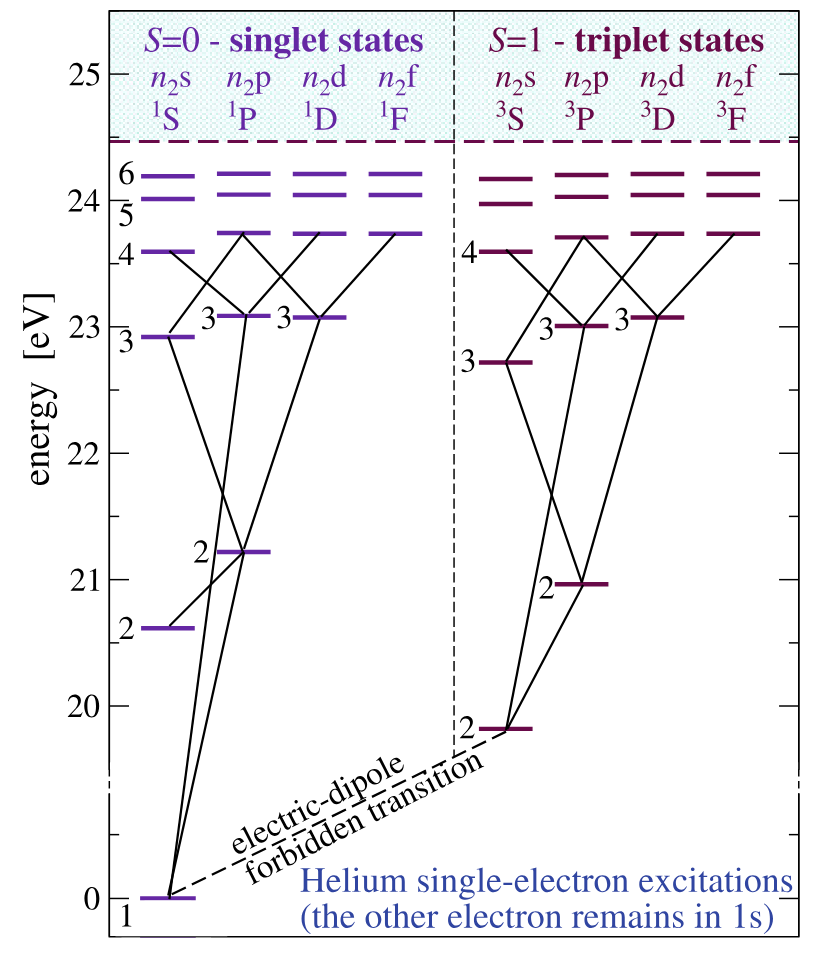
\includegraphics[width = 0.40 \textwidth]{ortho-para-he.png}
	\caption{Energy levels and electric-dipole transitions of atomic $ \ch{He} $.}
	\label{helium}
\end{figure}

\subsection{Elettroni interagenti}
\label{he-inter-electr}

Trattando in maniera perturbativa il potenziale d'interazione $ V_{ee} $, al prim'ordine si ha una correzione all'energia (nelle configurazioni para- o orto-) data da:
\begin{equation*}
	\begin{split}
		\Delta E_{k_1,k_2}^\text{(p,o)}
		& = \braket{\Psi_{k_1,k_2}^\text{(p,o)} | V_{ee} | \Psi_{k_1,k_2}^\text{(p,o)}} = \frac{e^2}{2} \int_{\R^6} \frac{d^3r_1 d^3r_2}{\abs{\ve{r}_1 - \ve{r}_2}}  \abs{\psi_{k_1}(\ve{r}_1) \psi_{k_2}(\ve{r}_2) \pm \psi_{k_1}(\ve{r}_2) \psi_{k_2}(\ve{r}_1)}^2 \\
		& = \frac{e^2}{2} \int_{\R^6} \frac{d^3r_1 d^3r_2}{\abs{\ve{r}_1 - \ve{r}_2}} \left[ \abs{\psi_{k_1}(\ve{r}_1)}^2 \abs{\psi_{k_2}(\ve{r}_2)}^2 + \abs{\psi_{k_1}(\ve{r}_2)}^2 \abs{\psi_{k_2}(\ve{r}_1)}^2 \right] \\
		& \quad \pm \frac{e^2}{2} \int_{\R^6} \frac{d^3r_1 d^3r_2}{\abs{\ve{r}_1 - \ve{r}_2}} \left[ \psi_{k_1}^*(\ve{r}_1) \psi_{k_2}^*(\ve{r}_2) \psi_{k_1}(\ve{r}_2) \psi_{k_2}(\ve{r}_1) + \psi_{k_1}(\ve{r}_1) \psi_{k_2}(\ve{r}_2) \psi_{k_1}^*(\ve{r}_2) \psi_{k_2}^*(\ve{r}_1) \right] \\
		& \equiv E_{k_1,k_2}^\text{(c)} \pm E_{k_1,k_2}^\text{(s)}
	\end{split}
\end{equation*}
dove $ k_i \equiv \{n_i,\ell_i,m_i\} $. $ E^\text{(c)} $ è l'energia dovuta all'interazione Coulombiana, mentre $ E^\text{(s)} $ è dovuta all'interazione di scambio: si dimostra che $ E^\text{(s)} \ge 0 $, dunque la configurazione para- ha un'energia superiore a quella orto- (come si vede in Fig. \ref{helium}). \\
Il fatto che la configurazione orto- sia energeticamente inferiore a quella para- può anche essere dedotto intuitivamente dalla simmetria della funzione d'onda: nel caso orto-, poiché la funzione d'onda spaziale è antisimmetrica, si ha $ \psi(\ve{r},\ve{r}) = 0 $, dunque è molto meno probabile che i due elettroni si trovino vicini rispetto al caso para-. Poiché $ V_{ee} \sim \abs{\ve{r}_1 - \ve{r}_2}^{-1} $, ciò significa che la correzione al prim'ordine dell'energia sarà maggiore nel caso para- rispetto a quello orto-. \\
Gli stati $ (n_1[\ell_1])(n_2[\ell_2]) $ subiscono dunque uno splitting energetico pari a $ 2E^\text{(s)}_{n_1,\ell_1 ; n_2,\ell_2} $ (la dipendenza da $ m $ c'è solo in presenza di campi elettromagnetici esterni che perturbano la simmetria sferica), noto come \textit{splitting da scambio}. Questo splitting è molto importante, poiché sta alla base della \textit{prima regola di Hund}: lo stato energeticamente più basso è sempre quello che massimizza lo spin\footnotemark.

\footnotetext{Ciò nel caso dell'atomo a 2 elettroni non ha alcun effetto sul ground state, poiché esso ha configurazione elettronica $ \text{1s}^2 $, dunque necessariamente $ S = 0 $.}

\section{Atomi ad \texorpdfstring{$ N $}{N} elettroni}

L'approccio perturbativo non dà un buon accordo coi dati sperimentali per $ N \ge 3 $: di conseguenza, è necessario adottare un altro metodo. Un'opzione è sfruttare il principio di Ritz (Th. \ref{th:ritz}): supponendo di avere un set di autofunzioni single-particle $ \{\phi_{\alpha_i}(w_i)\}_{i = 1, \dots, N} $ note, è possibile cercare un set di autofunzioni che fungono da base per lo spazio di Hilbert del sistema considerato andando a minimizzare il funzionale energia:
\begin{equation}
	E[\phi_{\alpha_1}, \dots, \phi_{\alpha_N}] = \frac{\braket{\Phi_{\alpha_1, \dots, \alpha_N} | \mathcal{H}_\text{MEA} | \Phi_{\alpha_1, \dots, \alpha_N}}}{\braket{\Phi_{\alpha_1, \dots, \alpha_N} | \Phi_{\alpha_1, \dots, \alpha_N}}}
	\label{eq:en-functional-def}
\end{equation}
dove $ \Phi_{\alpha_1, \dots, \alpha_N} $ è il determinante di Slater delle $ \{\phi_{\alpha_i}\}_{i = 1, \dots, N} $, le quali sono dette \textit{orbitali atomici}. Essendo $ \mathcal{H}_\text{MEA} = T + V_{ne} + V_{ee} $, si può esplicitare il funzionale come:
\begin{equation}
	\begin{split}
		E[\phi_{\alpha_1}, \dots, \phi_{\alpha_N}]
		& = \sum_{i = 1}^{N} \braket{\alpha_i | \mathcal{H}_0 | \alpha_i} \\
		& \quad + \frac{1}{2} \sum_{i,j = 1}^{N} \int dw\,dw'\, \abs{\phi_{\alpha_i}(w)}^2 v_{ee}(w,w') \abs{\phi_{\alpha_j}(w')}^2 \\
		& \quad - \frac{1}{2} \sum_{i,j = 1}^{N} \int dw\,dw'\, \phi_{\alpha_i}^*(w) \phi_{\alpha_i}(w') v_{ee}(w,w') \phi_{\alpha_j}^*(w') \phi_{\alpha_j}(w)
	\end{split}
	\label{eq:en-functional}
\end{equation}
dove si è assunta l'ortonormalità $ \braket{\alpha_i | \alpha_j} = \delta_{ij} $ e si sono definiti:
\begin{equation}
	\mathcal{H}_0(w) \equiv \left[ -\frac{\hbar^2}{2m_e} \lap_\ve{r} - \frac{Ze^2}{r} \right] \otimes \id_\text{spin}
	\qquad \qquad
	v_{ee}(w,w') \equiv \frac{e^2}{\abs{\ve{r} - \ve{r}'}} \otimes \id_\text{spin}
\end{equation}
Il primo termine del funzionale energia contiene il moto indipendente di ogni elettrone nel potenziale generato dal nucleo, il secondo termine contiene l'interazione Coulombiana tra ciascun elettrone ed la distribuzione di carica media dovuta a tutti gli elettroni, e il terzo termine è un termine di natura non-classica e non-locale dovuto all'antisimmetria per scambio: si noti che il secondo termine contiene anche un'interazione di ciascun elettrone con sé stesso, la quale non ha senso fisico, che viene giustamente cancellata da un addendo nel terzo termine.

\begin{theorem}{Equazione di Hartree-Fock}{eq-hf}
	Il set di autofunzioni $ \{\psi_{\alpha_i}\}_{i = 1, \dots, N} $ che minimizza il funzionale energia soddisfa:
	\begin{equation}
		\mathcal{H}_0(w) \psi_\alpha(w) + V_\text{Ha}(w) \psi_\alpha(w) - \int dw'\, V_\text{Fock}(w,w') \psi_\alpha(w') = E_\alpha \psi_\alpha(w)
	\end{equation}
	dove i potenziali di Hartree e Fock sono definiti come:
	\begin{equation}
		V_\text{Ha}(w) \defeq \int dw'\, \sum_\beta \abs{\phi_\beta(w')}^2 v_{ee}(w,w')
	\end{equation}
	\begin{equation}
		V_\text{Fock}(w,w') \defeq \sum_\beta \phi_\beta^*(w') \phi_\beta(w) v_{ee}(w,w')
	\end{equation}

	\tcblower

	\begin{proof}
		Partendo dall'Eq. \ref{eq:en-functional-def}, si noti che in generale:
		\begin{equation*}
			\frac{\pa E(p)}{\pa p_i} = \frac{\pa}{\pa p_i} \frac{N(p)}{D(p)} = 0
			\quad \Leftrightarrow \quad
			\frac{1}{D(p)} \frac{\pa N(p)}{\pa p_i} - \frac{N(p)}{D^2(p)} \frac{\pa D(p)}{\pa p_i}
			\quad \Leftrightarrow \quad
			\frac{\pa N(p)}{\pa p_i} = E(p) \frac{\pa D(p)}{\pa p_i}
		\end{equation*}
		Applicando la derivata funzionale $ \frac{\delta}{\delta \phi_\alpha^*(w)} $:
		\begin{equation*}
			\frac{\delta}{\delta \phi_\alpha^*(w)} \braket{\Phi_{\alpha_1, \dots, \alpha_N} | \mathcal{H}_\text{MEA} | \Phi_{\alpha_1, \dots, \alpha_N}} = E[\alpha_1, \dots, \alpha_N] \frac{\delta}{\delta \phi_\alpha^*(w)} \braket{\Phi_{\alpha_1, \dots, \alpha_N} | \Phi_{\alpha_1, \dots, \alpha_N}} = E_\alpha \phi_\alpha(w)
		\end{equation*}
		Si calcola la derivata funzionale per ogni termine dell'Eq. \ref{eq:en-functional}:
		\begin{equation*}
			\frac{\delta}{\delta \phi_\alpha^*(w)} \sum_{i = 1}^{N} \braket{\alpha_i | \mathcal{H}_0 | \alpha_i} = \sum_{i = 1}^{N} \delta_{\alpha_i,\alpha} \mathcal{H}_0(w) \phi_{\alpha_i}(w) = \mathcal{H}_0 \phi_\alpha(w)
		\end{equation*}
		\begin{equation*}
			\begin{split}
				\frac{\delta}{\delta \phi_\alpha^*(w)}
				& \frac{1}{2} \sum_{i,j = 1}^{N} \int dw\,dw'\, \abs{\phi_{\alpha_i}(w)}^2 v_{ee}(w,w') \abs{\phi_{\alpha_j}(w')}^2 \\
				& = \frac{1}{2} \sum_{i,j = 1}^{N} \int dw' \left[ \delta_{\alpha_i,\alpha} \phi_{\alpha_i}(w) \abs{\phi_{\alpha_j}(w')}^2 + \abs{\phi_{\alpha_i}(w)}^2 \delta_{\alpha_j,\alpha} \phi_{\alpha_j}(w) \right] v_{ee}(w,w') \\
				& = \sum_{i = 1}^{N} \int dw'\, \abs{\phi_{\alpha_i}(w')}^2 v_{ee}(w,w') \phi_\alpha(w)
			\end{split}
		\end{equation*}
		\begin{equation*}
			\begin{split}
				\frac{\delta}{\delta \phi_\alpha^*(w)}
				& \frac{1}{2} \sum_{i,j = 1}^{N} \int dw\,dw'\, \phi_{\alpha_i}^*(w) \phi_{\alpha_i}(w') v_{ee}(w,w') \phi_{\alpha_j}^*(w') \phi_{\alpha_j}(w) \\
				& = \sum_{i = 1}^{N} \int dw' \phi_{\alpha_i}^*(w') \phi_{\alpha_i}(w) v_{ee}(w,w') \phi_\alpha(w')
			\end{split}
		\end{equation*}
		Rinominando $ \phi_\alpha \equiv \psi_\alpha $ e $ \phi_{\alpha_i} \equiv \phi_\beta $ di ottiene la tesi.
	\end{proof}
\end{theorem}

Si vede che l'equazione HF dipende comunque da un set di autofunzioni $ \{\phi_\beta\} $ ignoto: la strategia di risoluzione consiste nell'assumere che $ \{\phi_\beta\} $ sia un set arbitrario di $ N $ autofunzioni single-particle, risolvere l'equazione HF, scegliere come autofunzioni $ \{\psi_\alpha\} $ le $ N $ soluzioni con autovalore energetico $ E_\alpha $ più basso (\textit{regola dell'Aufbau}) e confrontare i sets $ \{\phi_\beta\} $ e $ \{\psi_\alpha\} $: se essi non variano in maniera apprezzabile (autoconsistenza), si è trovata una soluzione (approssimata) del problema, altrimenti si reitera il processo, assumendo ora $ \{\phi_\beta\} \equiv \{\psi_\alpha\} $. Generalmente si raggiunge l'autoconsistenza in $ 10-100 $ iterazioni. \\
Si noti che non si possono fare assunzioni a priori sul potenziale autoconsistente $ V_\text{HF} $: in  generale, esso non avrà simmetria sferica. Ciò significa che $ E_\alpha $ non avranno l'andamento dell'Eq. \ref{eq:1-e-en}, ma in generale $ E_\alpha = E_{n,\ell} $: ciò spiega l'ordinamento energetico $ n\text{s} < n\text{p} < n\text{d} < \dots $ osservato per gli orbitali atomici.

\begin{example}{Ground state dell'Argon}{}
	La configurazione elettronica del ground state dell'$ \ch{Ar} $ ($ N = Z = 18 $) è data dalla regola dell'Aufbau e derivata dall'equazione HF: $ \text{1s}^2 \text{2s}^2 \text{2p}^6 \text{3s}^2 \text{3p}^6 $.
\end{example}

\subsection{Atomi idrogenoidi}

Il metodo HF è applicabile anche al caso di un atomo idrogenoide. In tal caso, si considera una generica combinazione di autofunzioni single-particle e si cercano i coefficienti che danno la miglior stima:
\begin{equation*}
	\Psi = \sum_\alpha c_\alpha \phi_\alpha
	\qquad \qquad
	E[\{c_\alpha\}] = \frac{\sum_{\alpha,\beta} c_\alpha^* c_\beta \braket{\phi_\alpha | \mathcal{H} | \phi_\beta}}{\sum_{\alpha,\beta} c_\alpha^* c_\beta \braket{\phi_\alpha | \phi_\beta}} = \frac{\sum_{\alpha,\beta} c_\alpha^* c_\beta \braket{\phi_\alpha | \mathcal{H} | \phi_\beta}}{\sum_\alpha \abs{c_\alpha}^2}
\end{equation*}
assumendo autofunzioni ortonormali $ \braket{\phi_\alpha | \phi_\beta} = \delta_{\alpha\beta} $. Applicando lo stesso ragionamento della dimostrazione del Th. \ref{th:eq-hf}:
\begin{equation*}
	\frac{\pa}{\pa c_k^*} \sum_{\alpha,\beta} c_\alpha^* c_\beta \braket{\phi_\alpha | \mathcal{H} | \phi_\beta} = E[\{c_\alpha\}] \frac{\pa}{\pa c_k^*} \sum_\alpha \abs{c_\alpha}^2
	\quad \Leftrightarrow \quad
	\braket{\phi_k | \mathcal{H} | \Psi} = E_k c_k = E_k \braket{\phi_k | \Psi}
\end{equation*}
L'equazione HF si riduce dunque all'equazione di Schrödinger $ \mathcal{H} \ket{\phi_k} = E_k \ket{\phi_k} $.

\subsection{Tavola periodica}

L'equazione HF permette di predire le configurazioni elettroniche degli elementi della tavola periodiche e le relative proprietà periodiche.

\subsubsection{Configurazioni elettroniche}

Negli elementi fino al $ \ch{Be} $ ($ N \le 4 $) il campo HF gode di simmetria sferica, poiché gli elettroni si dispongono su orbitali $ \text{s} $ perfettamente simmetrici. Per gli elementi successivi, la simmetria sferica è presente soltanto nei gas nobili. \\
Fino all'$ \ch{Ar} $ ($ Z = N = 18 $) gli orbitali vengono riempiti nel consueto ordine, ed infatti la sua configurazione elettronica è $ [\ch{Ar}] = \text{1s}^2 \text{2s}^2 \text{2p}^6 \text{3s}^2 \text{3p}^6 $. Da questo valore di $ Z $, però, la dipendenza di $ E_{n,\ell} $ da $ \ell $ si fa così forte da rendere $ E_\text{3d} > E_\text{4s} $: ciò è sperimentalmente confermato dalla configurazione atomica del potassio $ [\ch{K}] = [\ch{Ar}] \text{4s}^1 $. Dopo il riempimento della shell $ \text{4s} $ e prima di quello della $ \text{4p} $ avviene il riempimento della $ \text{3d} $: alcune inversioni (es.: $ \ch{Cr} $, $ \ch{Cu} $) mostrano come $ \text{3d} $ e $ \text{4s} $ siano energeticamente molto vicini, così da rendere importanti fenomeni di correlazione elettronica; fenomeni analoghi sono messi in luce anche nel riempimento delle shell $ \text{4d} $, $ \text{4f} $, $ \text{5d} $ e $ \text{5f} $.

\subsubsection{Proprietà periodiche}

L'andamento dell'energia di prima ionizzazione e del raggio atomico degli atomi neutri conferma l'organizzazioni in gruppi della tavola periodica: infatti, atomi con gli stessi elettroni di valenza tendono a comportarsi analogamente.

\begin{figure}
	\centering
	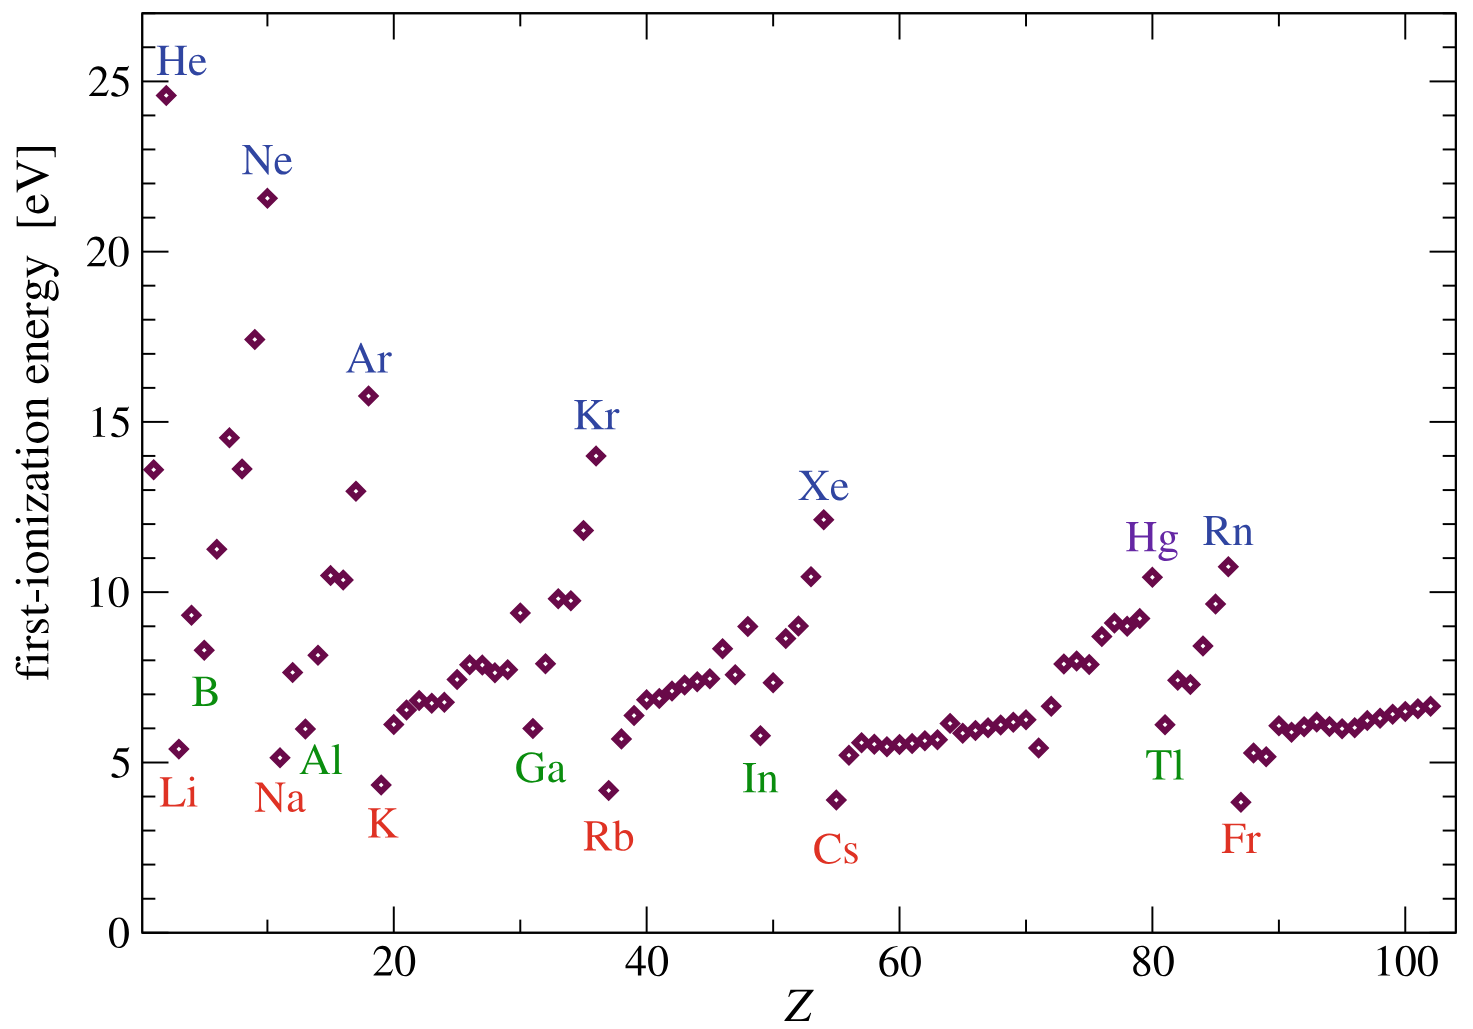
\includegraphics[width = 0.49 \textwidth]{ionization-energy.png}
	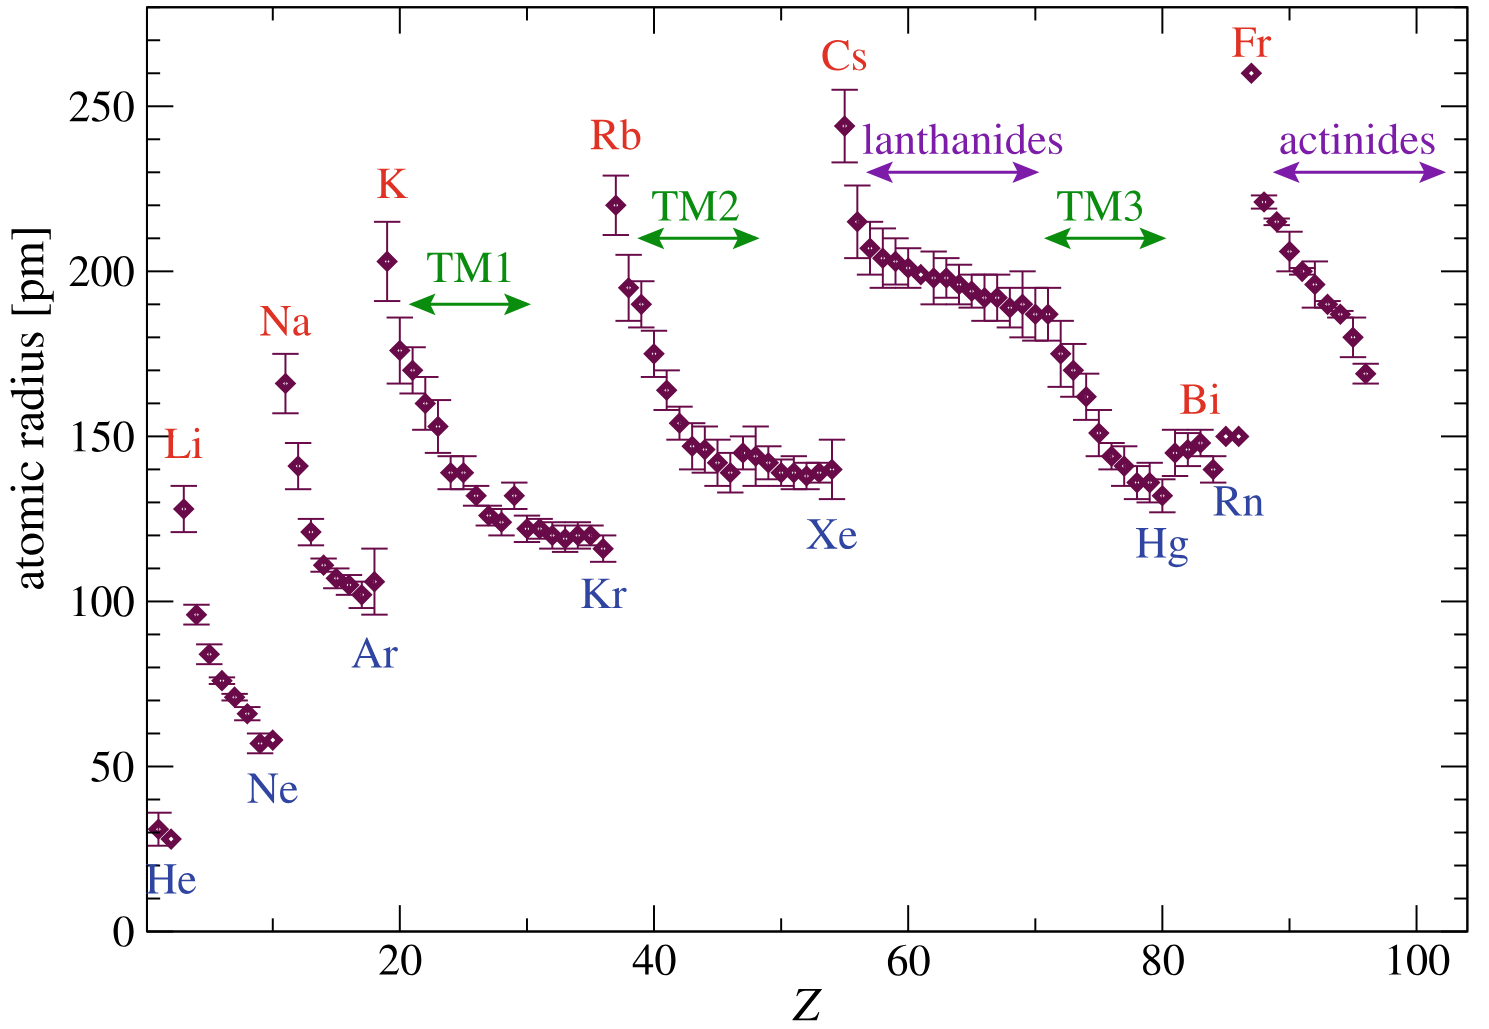
\includegraphics[width = 0.49 \textwidth]{atomic-radius.png}
	\caption{First ionization energy and atomic radius across the periodic table.}
	\label{ion-en-atom-rad}
\end{figure}

Come si può vedere in Fig. \ref{ion-en-atom-rad}, sperimentalmente viene confermato il fatto che i gas nobili hanno shell di valenza complete, poiché presentano energia di prima ionizzazione massima e raggio atomico minimo rispetto agli elementi del loro gruppo. Al contrario, i metalli alcalini hanno un solo elettrone di valenza, per di più molto distante dalle shell interne, come si evince da considerazioni analoghe. \\
Si vede inoltre che gli atomi con shell $ \text{d} $ o $ \text{f} $ incomplete tendono ad avere proprietà (a basse energie) piuttosto uniformi: vengono perciò ragguppati in metalli di transizione ($ \text{3d} $, $ \text{4d} $ e $ \text{5d} $), lantanidi ($ \text{4f} $) ed attinidi ($ \text{5f} $).

\begin{example}{Energia di prima ionizzazione dell'elio}{}
	Se si considera l'$ \ch{He} $, dallo studio della sua energia di ionizzazione si vede come sia necessario considerare l'interazione tra elettroni. Mentre l'energia del catione $ \ch{He}^+ $ è calcolabile usando lo spettro idrogenoide (Eq. \ref{eq:1-e-en}), trovando $ E(\ch{He}^+) = -54\ev $, se si usasse quest'ultimo per calcolare anche l'energia di $ \ch{He} $ si troverebbe $ E(\ch{He}) = 2 E(\ch{He}^+) = - 108\ev $, per un'energia di prima ionizzazione $ E_1(\ch{He}) = 54\ev $ in contrasto col dato sperimentale $ E_1(\ch{He}^+) \simeq 24\ev $. Tenendo conto dell'interazione elettronica, ovvero della correzione in Sec. \ref{he-inter-electr}, si trova $ E(\ch{He}) = -77.8\ev $, ovvero $ E_1(\ch{He}) = 24.2\ev $, dunque in perfetto accordo con le osservazioni.
\end{example}

\subsubsection{Regole di Hund}

Per ottenere la configurazione elettronica del ground state (o degli stati eccitati) di un atomo è necessario svolgere la trattazione HF completa. È però possibile approssimare il risultato utilizzando delle regole semi-empiriche, dette regole di Hund, per stabilire quale, tra tutti gli stati possibili\footnotemark, è il ground state; in ordine d'importanza:
\begin{enumerate}
	\item massimizzare lo spin totale $ \bs{S} $;
	\item massimizzare il momento angolare orbitale totale $ \bs{L} $;
	\item per il momento angolare totale $ \bs{J} $, in base al riempimento della shell:
		\begin{itemize}
			\item se è meno di semipiena, minimizzare $ \bs{J} $;
			\item se è più di semipiena, massimizzare $ \bs{J} $.
		\end{itemize}
\end{enumerate}
Queste regole si basano sul minimizzare l'energia del sistema. Per quanto riguarda la prima regola, gli stati atomici a spin più basso hanno energia maggiore poiché, essendo il moto degli elettroni poco correlato, questi tendono a trovarsi in media vicini gli uni agli altri più spesso rispetto agli stati atomici a spin più alto, risultando in una maggiore energia Coulombiana. \\
La seconda regola, invece, deriva dal fatto che, a parità di spin, gli elettroni si evitano più efficientemente quando ruotano in maniera coordinata, ovvero in stati atomici ad alto momento angolare orbitale (a parità di spin, massimizzato dalla prima regola). \\
Infine, massimizzati $ \bs{S} $ ed $ \bs{L} $, rimane da determinare $ \bs{J} $ (poiché $ \bs{S} $ ed $ \bs{L} $ vengono accoppiati dall'interazione spin-orbita): lo stato ad energia minore viene determinato dal segno del coefficiente spin-orbita. Se si considera una shell meno che semipiena, questo sarà naturalmente positivo, ma, se si considera una shell più che semipiena, gli elettroni mancanti possono essere interpretati come particelle di carica opposta, così da avere:
\begin{equation*}
	\mathcal{H}_\text{s-o} = \xi_{n,\ell} \sum_{i = 1}^{n_e} \bs{s}_i \cdot \bs{\ell}_i = \xi_{n,\ell} \underbrace{\sum_{i = 1}^{t} \bs{s}_i \cdot \bs{\ell}_i}_{0} - \xi_{n,\ell} \sum_{i = n_e+1}^{t} \bs{s}_i \cdot \bs{\ell}_i = - \xi_{n,\ell} \sum_{i = n_e + 1}^{t} \bs{s}_i \cdot \bs{\ell}_i
\end{equation*}
Dunque, si vede che nelle shell meno che semipiene va minimizzato $ \bs{J} $, mentre in quelle più che semipiene esso va massimizzato. \\
Si noti che queste regole hanno natura fenomenologica e, sebbene risultino alquanto accurate nel predire i ground states atomici, risultano molto spesso fallaci nella trattazione degli stati eccitati.

\footnotetext{In questo caso, si considerano solo i microstati associati all'ultima shell non completamente riempita: detti $ t $ il numero massimo di elettroni allocabili in tale shell ed $ n_e $ il numero di elettroni da collocarvi, il numero totale di microstati possibili è $ \binom{t}{n_e} $.}

\paragraph{Coupling schemes}

Le regole di Hund si basano sul cosiddetto \textit{Russell-Saunders coupling}, il quale prevede che vengano prima vengano accoppiati i vari $ \bs{s}_i $ a dare $ \bs{S} $ ed i vari $ \bs{\ell}_i $ a dare $ \bs{L} $, e successivamente $ \bs{S} $ ed $ \bs{L} $ vengano accoppiati a dare $ \bs{J} $. Questo coupling scheme risulta efficace in atomi a basso $ Z $, in cui il potenziale HF (Coulombiano + scambio) è dominante rispetto a quello spin-orbita. \\
Al contrario, per atomi con $ Z \ge 50 $ il potenziale spin-orbita diventa dominante\footnotemark: in questo caso, è necessario prima accoppiare i vari $ \bs{s}_i $ e $ \bs{\ell}_i $, ottenendo i $ \bs{j}_i $ individuali, e poi accoppiare quest'ultimi per ottenere $ \bs{J} $. Questo è noto come \textit{jj coupling}. \\
Mentre la base LS è quasi-diagonale per basso $ Z $ e quella jj lo è per alto $ Z $, a $ Z $ intermedi è necessario diagonalizzare opportunamente sia il termine Coulombiano che quello di spin-orbita.

\footnotetext{Mentre l'energia d'interazione spin-orbita cresce all'aumentare di $ Z $, l'energia d'interazione Coulombiana rimane pressoché costante, risultando addirittura attenuata dal progressivo allontanamento degli elettroni di valenza dal nucleo.}

\section{Spettroscopia}

\subsection{Transizioni di dipolo elettrico}

Nel caso di un sistema ad $ N $ elettroni, l'operatore dipolo elettrico è definito come la somma degli operatori single-particle:
\begin{equation}
	\ve{d} \defeq \sum_{i = 1}^{N} \ve{d}_i = - q_e \sum_{i = 1}^{N} \ve{r}_i
\end{equation}

\begin{proposition}{Transizioni di dipolo elettrico}{}
	Nei sistemi ad $ N $ elettroni, le transizioni di dipolo elettrico sono realizzate da un \textit{singolo elettrone} che transisce, mentre gli altri rimangono nello stato single-particle iniziale.

	\tcblower

	\begin{proof}
		Nell'approssimazione HF di campo medio:
		\begin{equation*}
			\begin{split}
				& {^\text{(a)}\langle} \beta_1, \dots, \beta_N | \sum_{i = 1}^{N} \ve{d}_i | \alpha_1, \dots, \alpha_N {\rangle^\text{(a)}} = \\
				& \qquad \qquad \qquad = \frac{1}{N!} \sum_{i = 1}^{N} \sum_{\pi,\rho \in S^N} (-1)^{\{\pi\} + \{\rho\}} \braket{\beta_{\pi(1)} | \alpha_{\rho(1)}} \dots \braket{\beta_{\pi(i)} | \ve{d}_i | \alpha_{\rho(i)}} \dots \braket{\beta_{\pi(N)} | \alpha_{\rho(N)}} \\
				& \qquad \qquad \qquad = \frac{1}{N!} \sum_{i = 1}^{N} \sum_{\pi,\rho \in S^N} (-1)^{\{\pi\} + \{\rho\}} \braket{\beta_{\pi(i)} | \ve{d}_i | \alpha_{\rho(i)}} \prod_{j \neq i} \delta_{\beta_{\pi(j)} , \alpha_{\rho(j)}}
			\end{split}
		\end{equation*}
		Si noti che queste $ N - 1 $ delta di Kronecker fissano completamente la permutazione $ \rho \equiv \pi $, dunque:
		\begin{equation*}
			\begin{split}
				{^\text{(a)}\langle} \beta_1, \dots, \beta_N | \sum_{i = 1}^{N} \ve{d}_i | \alpha_1, \dots, \alpha_N {\rangle^\text{(a)}}
				& = \frac{1}{N!} \sum_{i = 1}^{N} \sum_{\pi \in S^N} \braket{\beta_{\pi(i)} | \ve{d}_i | \alpha_{\pi(i)}} \prod_{i \neq j} \delta_{\beta_{\pi(j)} , \alpha_{\pi(j)}} \\
				& = \sum_{i = 1}^{N} \braket{\beta_i | \ve{d}_i | \alpha_i} \prod_{j \neq i} \delta_{\beta_j , \alpha_j}
			\end{split}
		\end{equation*}
		Ciò equivale alla tesi.
	\end{proof}
\end{proposition}

Dato che le transizioni di dipolo-elettrico di un sistema ad $ N $ elettroni si riducono a quelle single-particle, si ha che le transizioni ammesse sono quelle in cui la configurazione elettronica dell'atomo cambia per un solo elettrone, tale per cui $ \Delta \ell_i = \pm 1 $ (più le altre condizioni in Eq. \ref{eq:1-e-el-dip-tr-m}-\ref{eq:1-e-el-dip-tr-spin}).

\begin{example}{Transizioni di dipolo elettrico del berillio}{}
	La configurazione elettronica del ground state del berillio è $ [\ch{Be}] = \text{1s}^2 \text{2s}^2 $. Possibili transizioni di dipolo elettrico ammesse sono $ \text{1s}^2 \text{2s}^2 \rightarrow \text{1s}^2 \text{2s}^1 \text{2p}^1 $ o $ \text{1s}^1 \text{2s}^2 \text{2p}^1 \rightarrow \text{1s}^1 \text{2s}^2 \text{4d}^1 $; transizioni proibite sono invece $ \text{1s}^2 \text{2s}^2 \rightarrow \text{1s}^2 \text{2s}^1 \text{3d}^1 $ o $ \text{1s}^2 \text{2s}^2 \rightarrow \text{1s}^1 \text{2s}^1 \text{2p}^1 \text{3p}^1 $.
\end{example}

\subsection{Eccitazioni di core}

Secondo la teoria HF, gli stati di core (single-particle), ovvero tutti gli elettroni non di valenza, subiscono una schermatura del potenziale del nucleo trascurabile, dunque la loro energia è molto negativa ($ \propto - Z^2 $): ciò è confermato dal fatto che, se per esempio si considera un eccitazione del $ \ch{Na} $ del tipo $ \text{1s}^2 \text{2s}^2 \text{2p}^6 \text{3s}^1 \rightarrow \text{1s}^1 \text{2s}^2 \text{2p}^6 \text{3s}^2 $, sono necessarie energie dell'ordine $ \sim 1\kev $ per eccitare gli stati di core al primo stato eccitato disponibile (a causa del principio d'esclusione). \\
Ne consegue che, data la dipendenza del decay rate da $ E_\text{if}^3 $, le eccitazioni di core presentano delle linee spettrali estremamente allargate, oltre $ \hbar \gamma \sim 1\ev $. Inoltre, dall'Eq. \ref{eq:electric-dipole-decay-rate}, si vede che $ \gamma \sim Z^4 $.

\begin{figure}
	\centering
	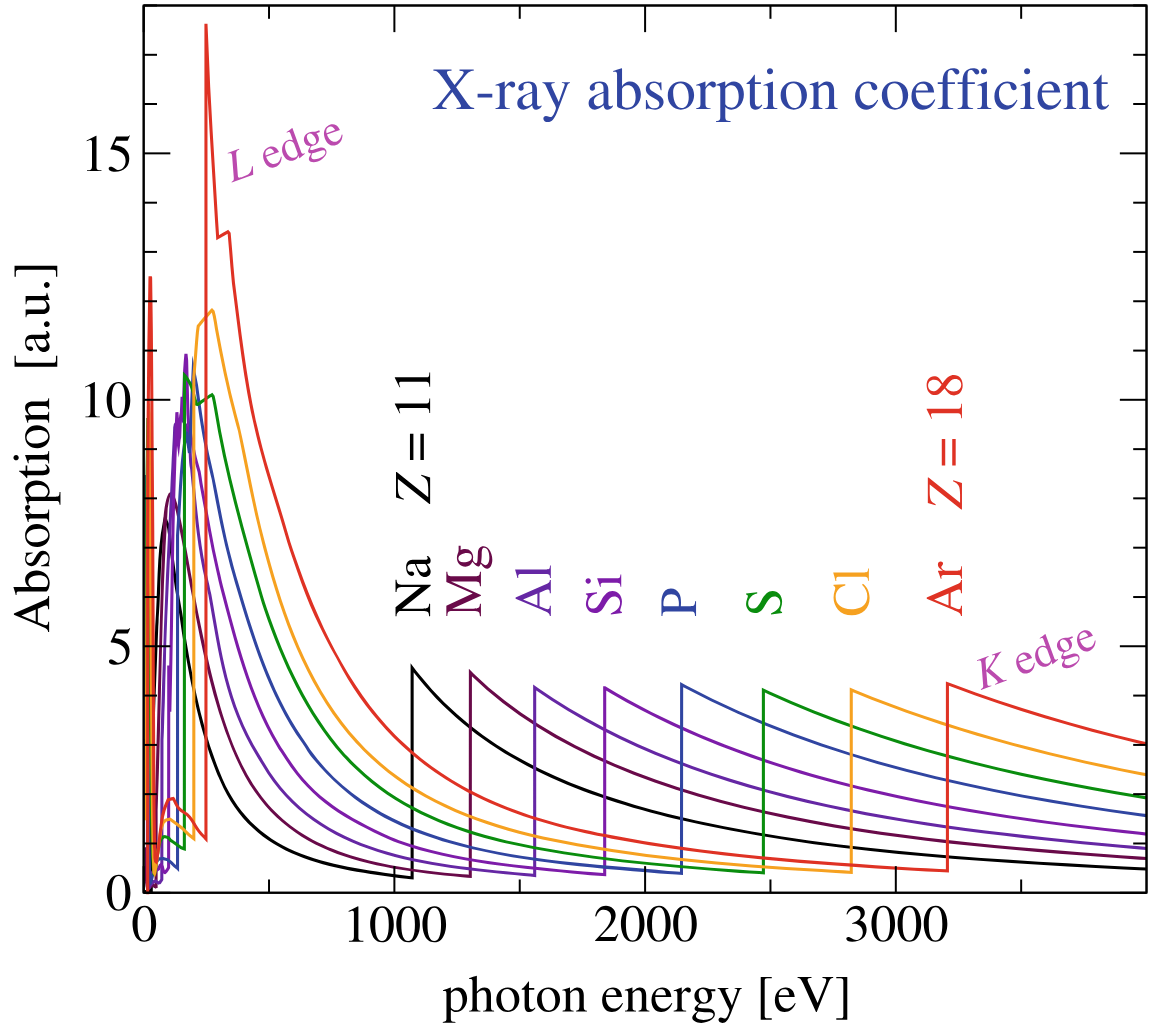
\includegraphics[width = 0.45 \textwidth]{core-exc-x-rays.png}
	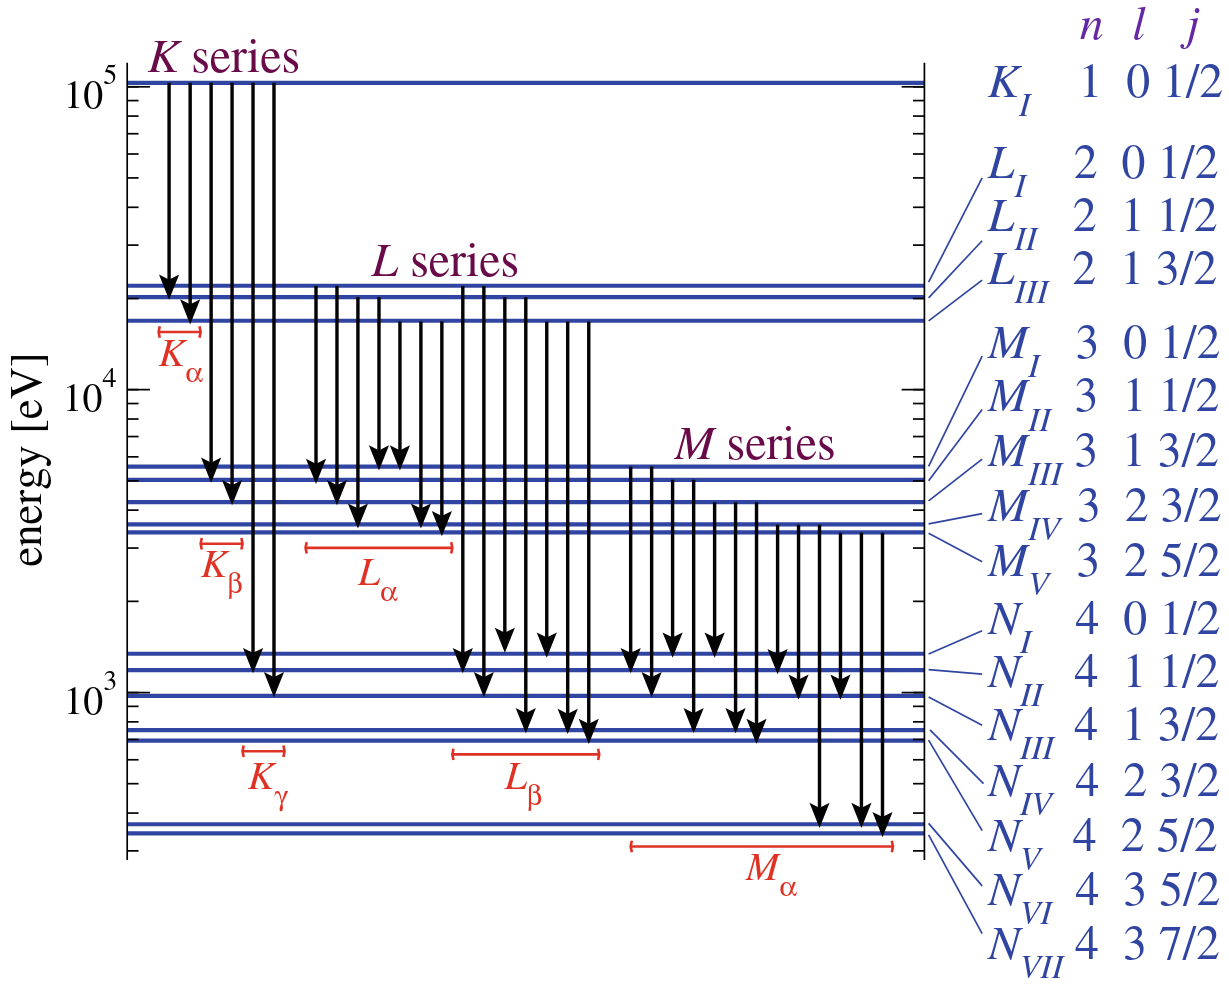
\includegraphics[width = 0.45 \textwidth]{core-exc-spectr.png}
	\caption{Observed X-ray absorption for third-period elements and observed core-level structure of $ \ch{U} $.}
	\label{core-exc}
\end{figure}

Le eccitazioni di core sono molto studiate a livello sperimentale: as esempio, i dati relativi all'assorbimento di raggi X (Fig. \ref{core-exc}) mostrano una certa regolarità per $ E_\gamma > 50\ev $, con un andamento sistematico rispetto a $ Z $. In particolare, si vede che negli spettri d'assorbimento di raggi X i picchi hanno una forma asimmetrica: per quanto riguarda l'estremità energeticamente inferiore, non può avvenire alcun assorbimento, in quanto l'energia non sarebbe sufficiente ad eccitare l'elettrone di core al primo stato eccitato libero (e, per il principio d'esclusione, esso non può essere eccitato a nessuno stato al di sotto di questo); superata la soglia d'assorbimento, invece, l'elettrone può essere eccitato a vari stati non-occupati, sia legati che non, risultando in uno spettro d'assorbimento continuo. \\
Si noti, inoltre, che all'aumentare dell'energia del fotone assorbito aumenta anche l'energia cinetica dell'elettrone ($ K_e = E_\gamma - E_\text{exc} $): conseguentemente, lo stato eccitato finale diventa progressivamente più ortogonale a quello iniziale. Ciò determina una rapida diminuzione di $ \gamma_\text{if} \propto \braket{\text{i} | \ve{d} | \text{f}} $, ovvero un rallentamento del decadimento. Per lo stesso motivo, inoltre, si capisce perché l'assorbimento di raggi X genera eccitazioni di core: se il fotone fosse assorbito da un elettrone di valenza, il quale è debolmente legato, la sua energia cinetica sarebbe molto alta, rendendo lo stato eccitato molto ortogonale rispetto a quello iniziale e rendendo $ \gamma $ trascurabile.

\subsubsection{Legge di Moseley}

Per quanto riguarda le transizioni tra stati di core, si adotta la seguente notazione: un \textit{hole} (elettrone mancante) in una shell $ n = 1,2,3,4,\dots$ è indicato da $ K,L,M,N,\dots $, mentre il numero di salti di shell è indicato da $ \alpha,\beta,\gamma,\dots$.

\begin{example}{Transizioni di core}{}
	Una transizione del tipo $ \text{1s}^1 \text{2s}^2 \text{2p}^6 \dots \rightarrow \text{1s}^2 \text{2s}^2 \text{2p}^5 \dots $ è indicata come $ K_\alpha \equiv K \rightarrow L $. Una transizione del tipo $ \text{1s}^2 \text{2s}^2 \text{2p}^5 \text{3s}^2 \text{3p}^6 \text{4s}^2 \dots \rightarrow \text{1s}^2 \text{2s}^2 \text{2p}^6 \text{3s}^2 \text{3p}^6 \text{4s}^1 \dots $ è $ L_\beta \equiv L \rightarrow N $.
\end{example}

Per quanto riguarda le linee spettrali $ K_\alpha $, dai dati sperimentali si evince una legge fenomenologica, detta \textit{legge di Moseley}:
\begin{equation}
	\frac{1}{\lambda_{K_\alpha}} \approx C \left( Z - a \right)^2
\end{equation}
dove $ C \approx \frac{3}{8} \frac{E_\text{Ha}}{2\pi \hbar c} \simeq 8.25 \cdot 10^6 \,\text{m}^{-1} $ ed $ a $ è il \textit{parametro di screening}. Quest'ultimo tiene conto dello screening che la carica nucleare subisce a causa degli elettroni di core (vedere Fig. \ref{screening}): non c'è una definizione ben precisa di $ a $, in quanto è un parametro fenomenologico, ma un buon accordo coi dati sperimentali è dato dal numero di elettroni nelle shell più interne a quelle considerate, includendo anche quella in esame (dunque $ (n,a) = (1,2) , (2,10), (3,28), \dots $).

\begin{figure}
	\centering
	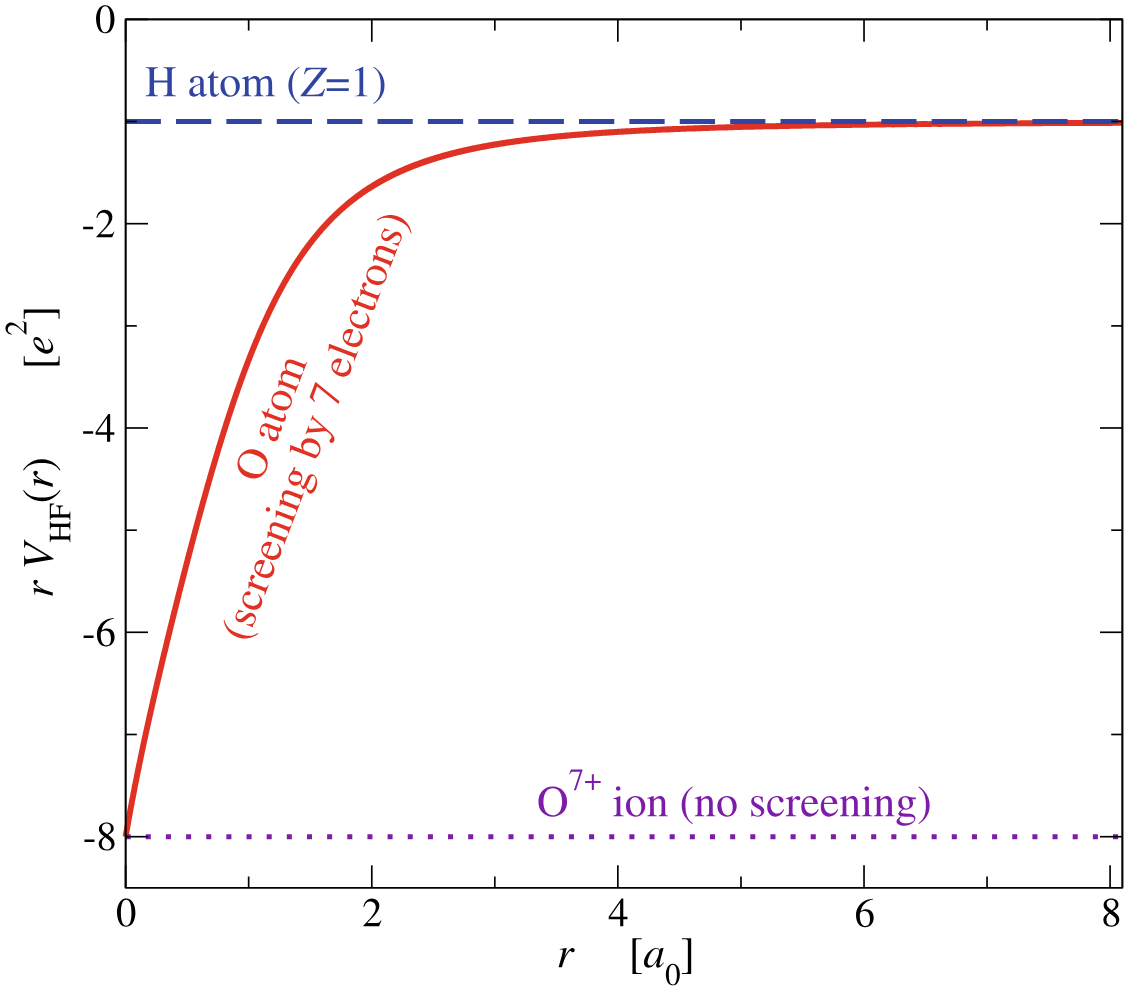
\includegraphics[width = 0.50 \textwidth]{screening.png}
	\caption{HF effective potential for atomic $ \ch{O} $ ($ N = Z = 8 $).}
	\label{screening}
\end{figure}

\subsection{Campo magnetico esterno}

Quando viene applicato un campo magnetico ad un MAE, si osserva un comportamento diverso in base alla presenza o meno di un momento magnetico. \\
Se si considera un atomo con $ J = 0 $, esso non ha alcun momento magnetico permanente: il campo esterno induce un piccolo momento magnetico $ \mu \sim \mu_\text{B} \frac{\mu_\text{B} B}{\Delta} $, dove $ \Delta $ è la differenza energetica tra il ground state ed il primo stato eccitato con $ J \neq 0 $, ma questi effetti sono trascurabili. \\
Al contrario, atomi con $ J \neq 0 $ hanno un momento magnetico permanente:
\begin{equation}
	\bs{\mu} = - g_J \mu_\text{B} \bs{J}
\end{equation}
dove $ g_J $ è il fattore di Landé (Eq. \ref{eq:lande-g-factor} con $ S,L,J $, nel LS coupling). Questo momento magnetico è rilevante nel limite Zeeman di campo esterno debole, che nella pratica è quello più importante in quanto difficilmente in laboratorio di riescono a produrre campi magnetici tali da dominare sull'interazione spin-orbita. \\
Per quanto riguarda lo splitting delle linee spettrali, si distingue tra \textit{regular Zeeman splitting}, nel caso in cui esse vengano splittate regolarmente in $ 2J + 1 $ linee spettrali (quando i fattori di Landé dello stato iniziale e finale sono uguali), e \textit{anomalous Zeeman splitting}, nel caso in cui lo splitting pattern sia più complesso (quando i fattori di Landé dello stato iniziale e finale sono diversi). \\
Un importante strumento sperimentale per studiare la degenerazione dei ground states dei MAE è l'apparato di Stern-Gerlach, nel quale gli atomi vengono deflessi (Eq. \ref{eq:stern-gerlach}) secondo:
\begin{equation*}
	F_z = \mu_z \frac{\pa B_z}{\pa z} = - g_J \mu_\text{B} M_J \frac{\pa B_z}{\pa z}
\end{equation*}
Il numero di sotto-fasci in cui viene splittato il fascio iniziale dà dunque una misura diretta dei possibili valori di $ M_J $, ovvero della degenerazione $ 2J + 1 $ del ground state.










